\section*{Supporting Information}
\renewcommand\thefigure{S\arabic{figure}}    
\setcounter{figure}{0}


\begin{figure}
  \begin{center}
    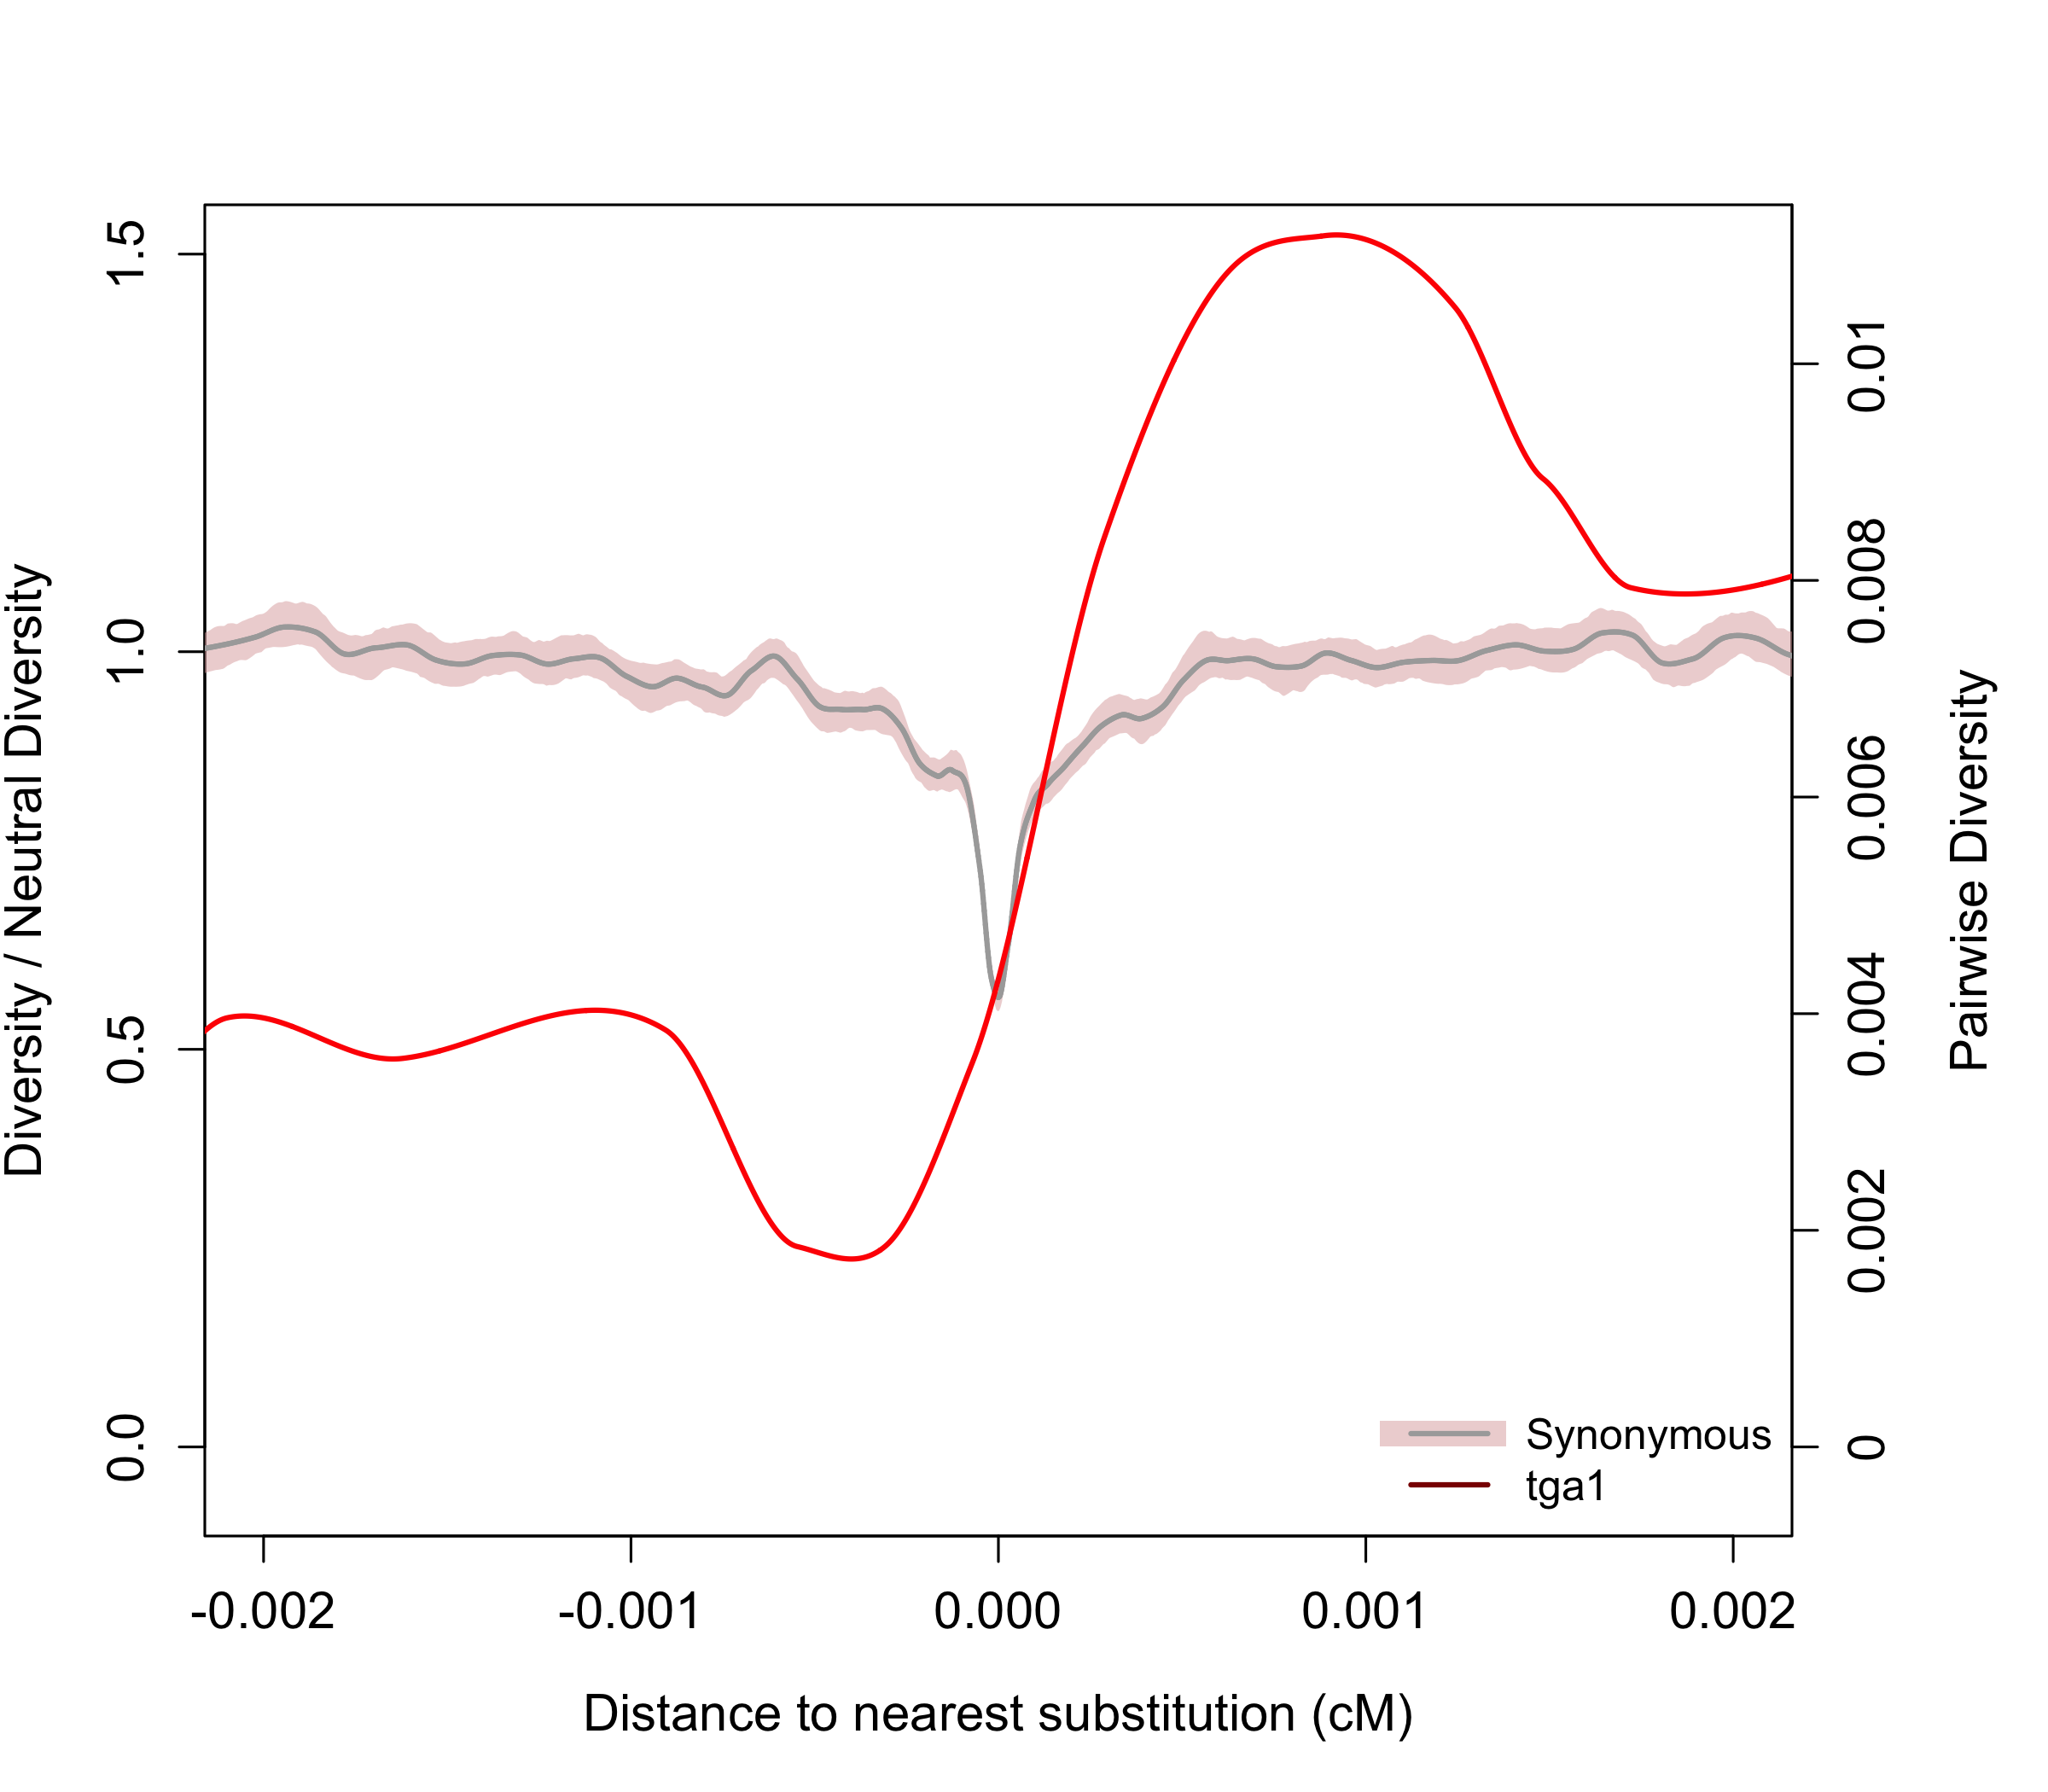
\includegraphics[width=.85\textwidth]{FigsAndFiles/plotDiversity_TvM_Folded2_Significance_tga1Supp_June.png} \\
    \end{center}
\caption{Diversity surrounding the causitive polymorphism at the \emph{tga1} locus is plotted. Since this is only one gene, the large amount of noise compared to our average plots is expected. However, notice that diversity precisely at the causitive polymorphism is reduced and a recovery of diversity is observed away from that site. \label{sFig:tga1}}
\end{figure}
\clearpage

\begin{figure}
  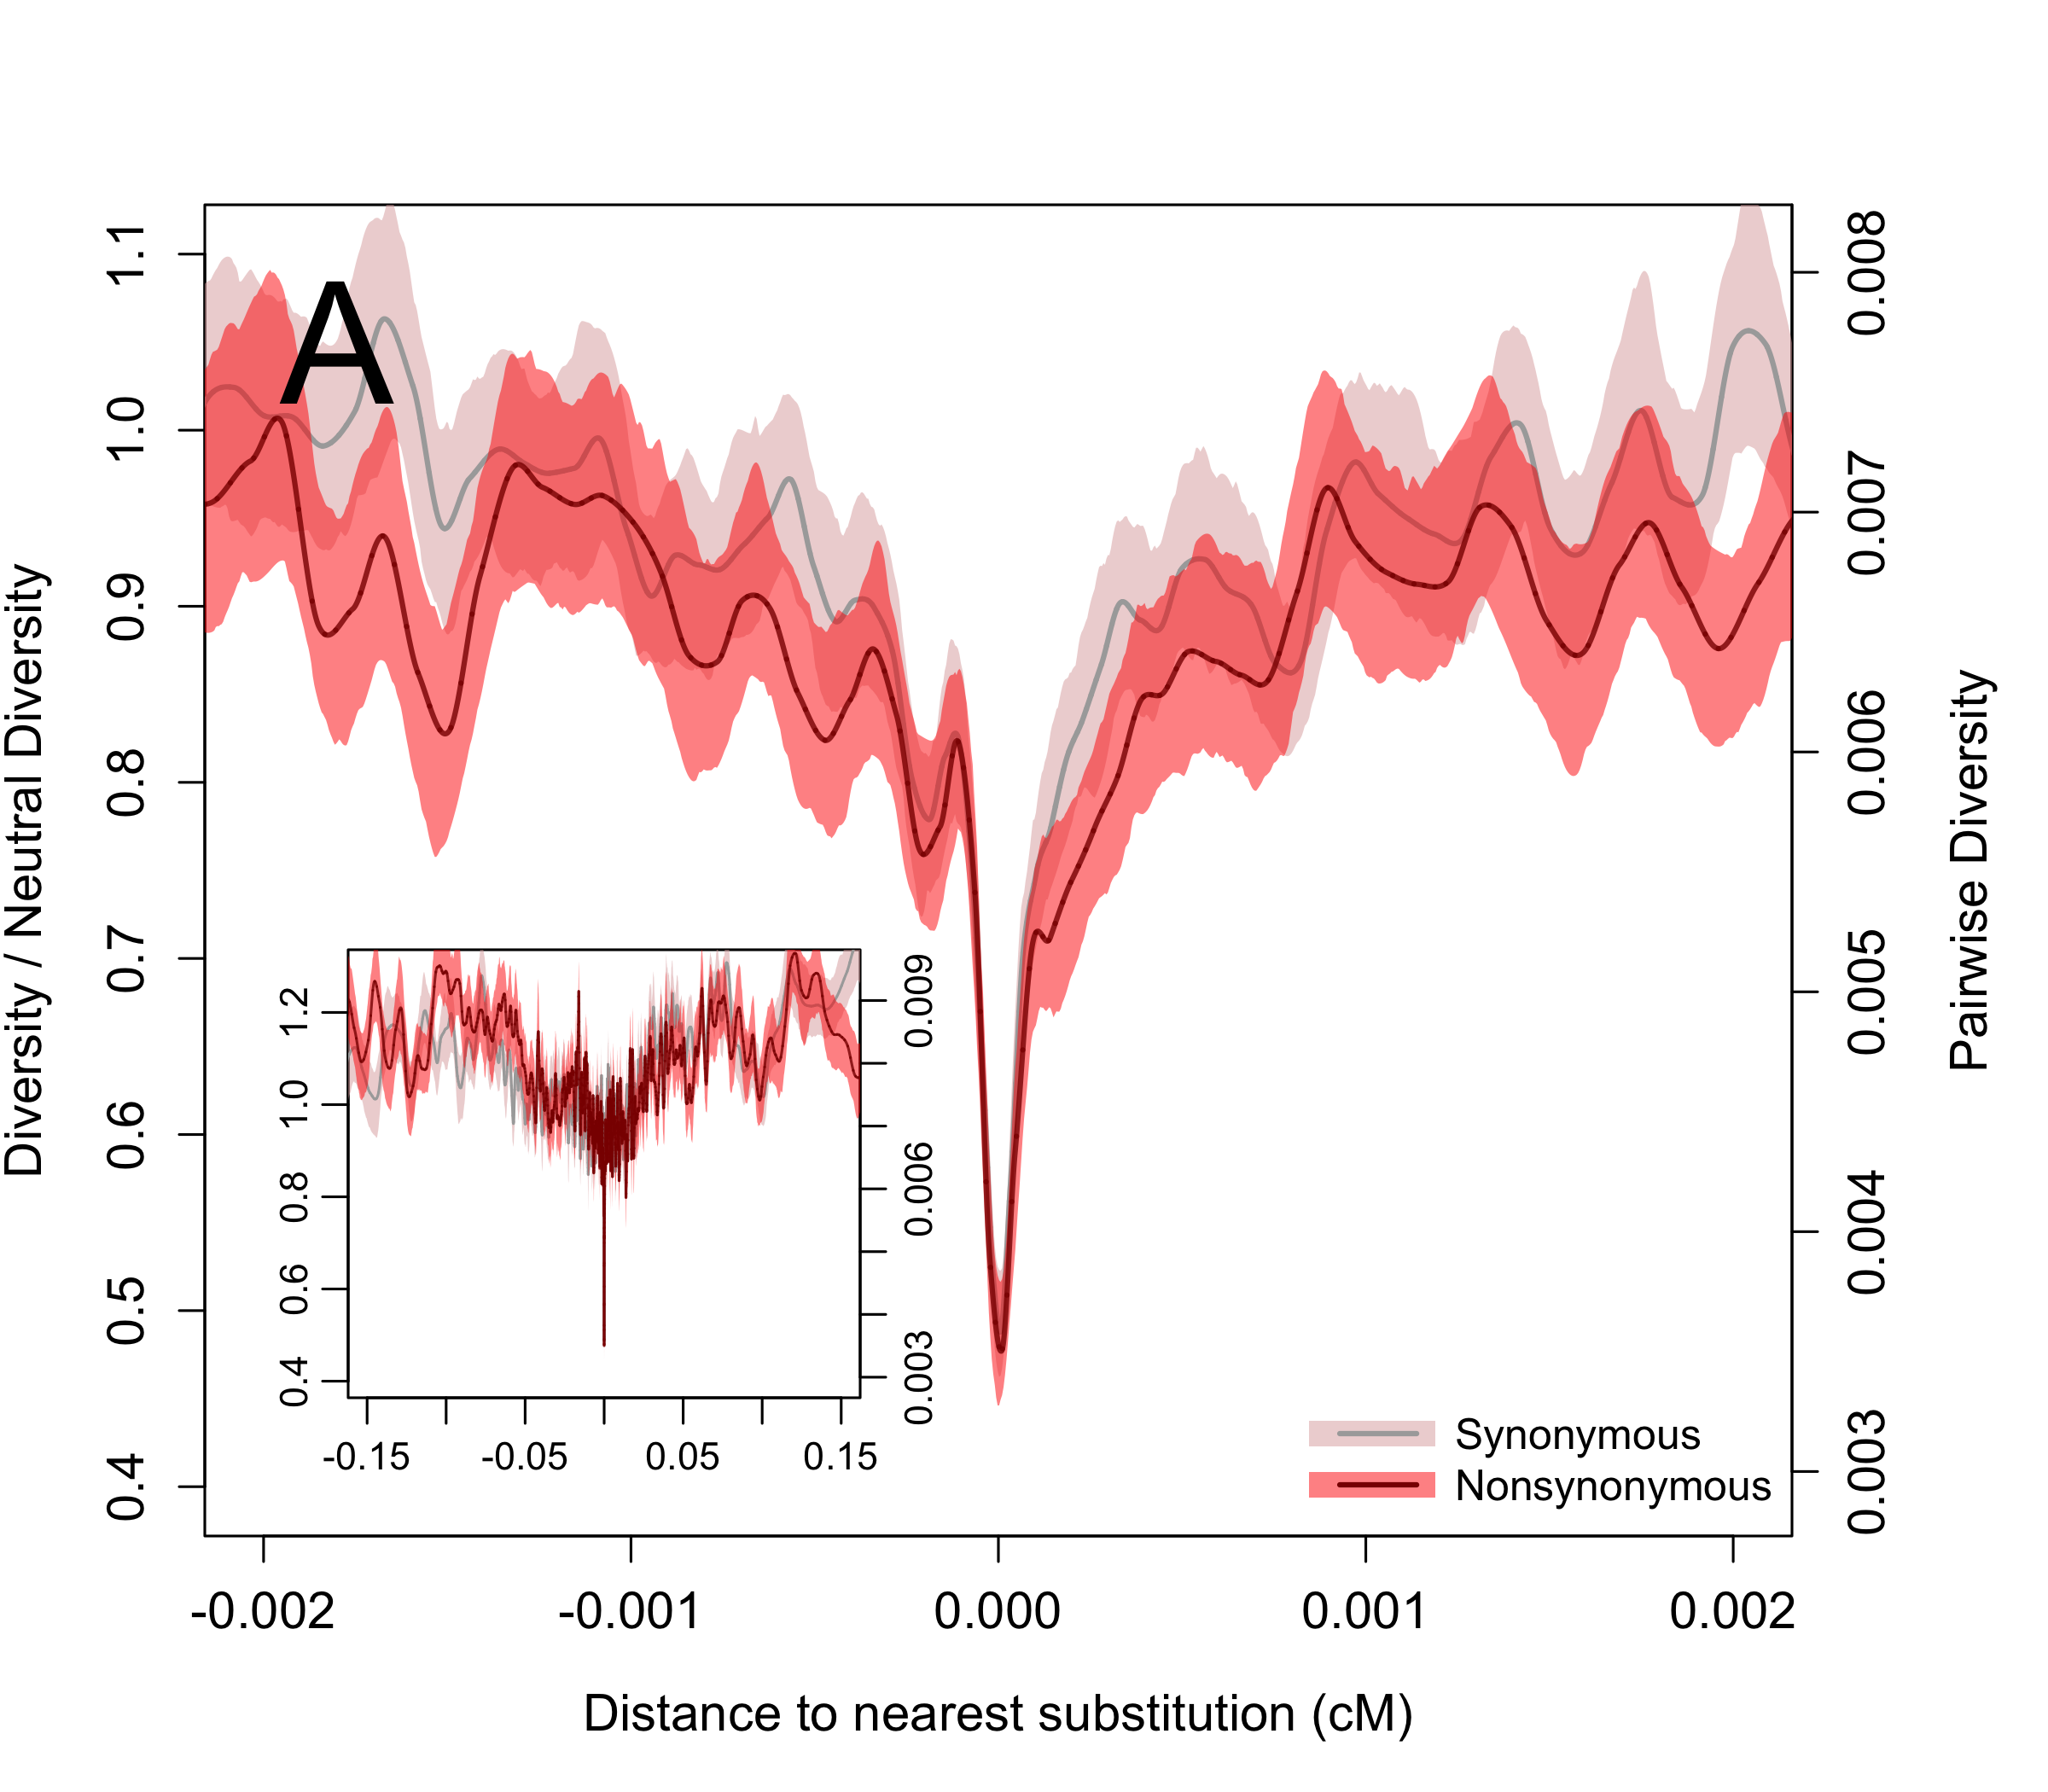
\includegraphics[width=.5\textwidth]{FigsAndFiles/plotDiversity_TvM_Conserved_Significance_June.png}
  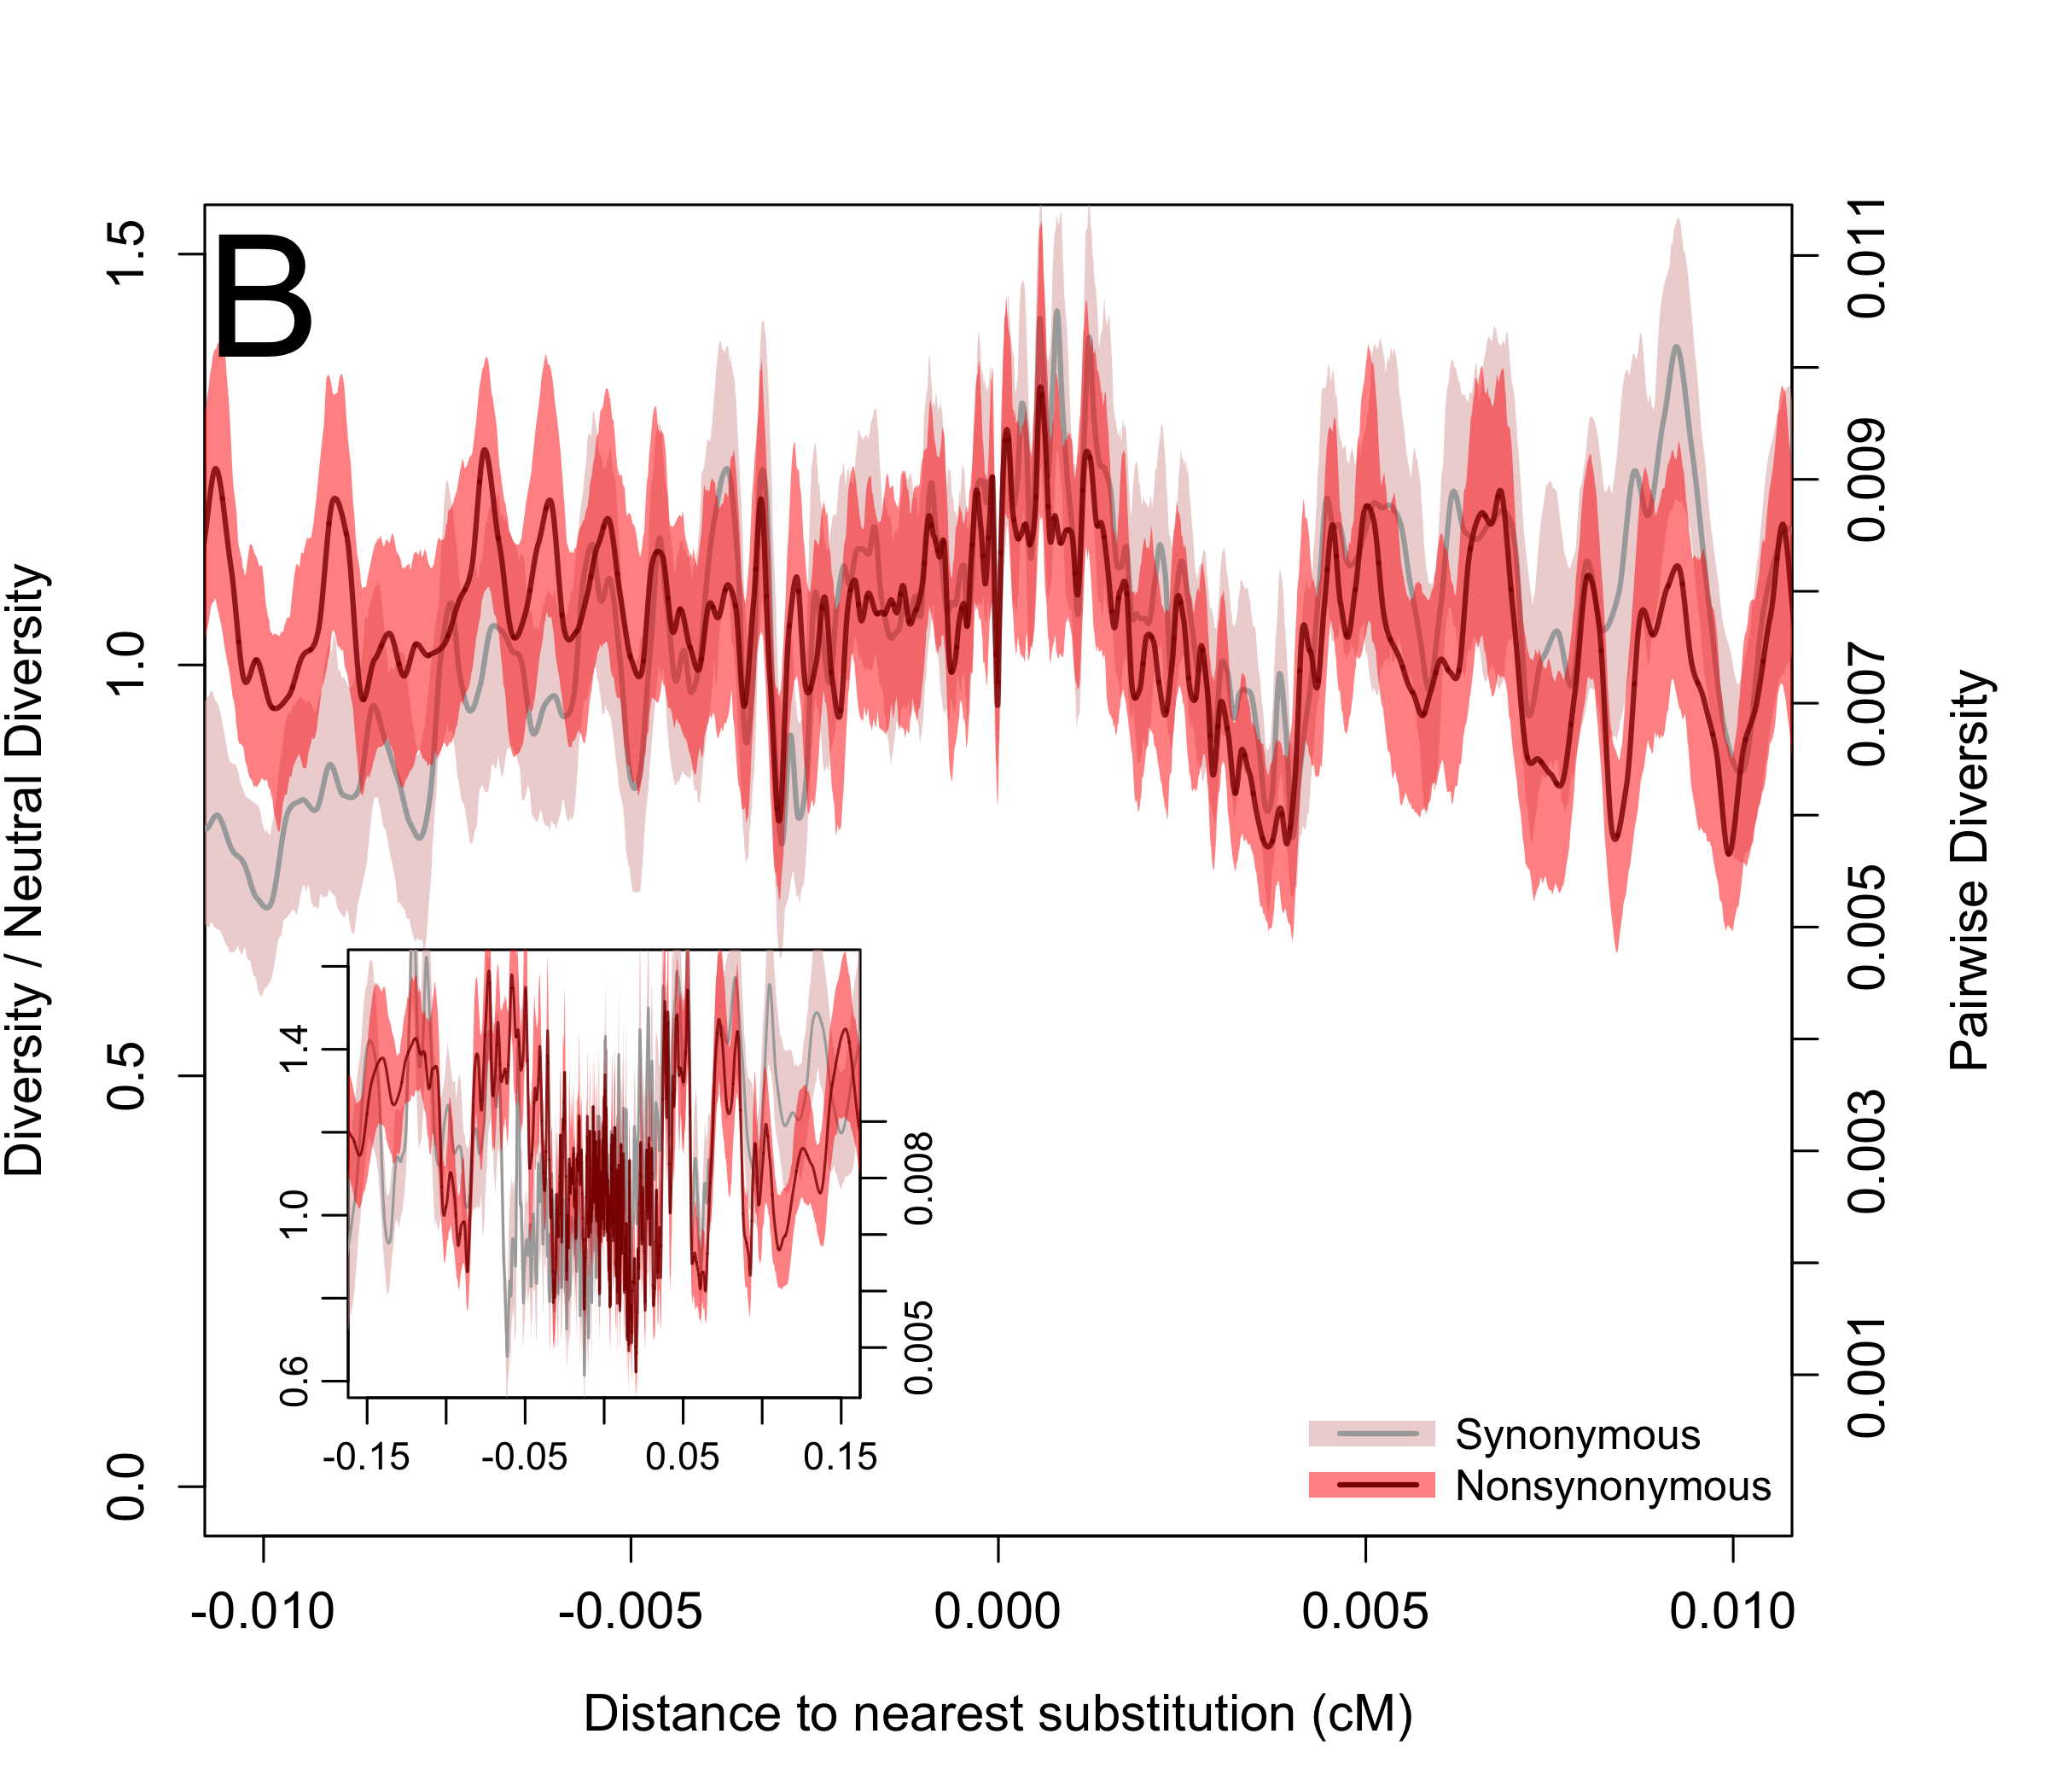
\includegraphics[width=.5\textwidth]{FigsAndFiles/plotDiversity_TvM_Unconserved_Significance_June.png}
\caption{ Pairwise diversity surrounding synonymous and nonsynonymous
  substitutions in maize at highly conserved (A) or unconserved (B) sites.  Bootstrap-based 95\% confidence intervals are depicted via shading. Inset plots depict a larger range on the x-axis. \label{sFig:consUncons}}
\end{figure}
\clearpage

\begin{figure}
  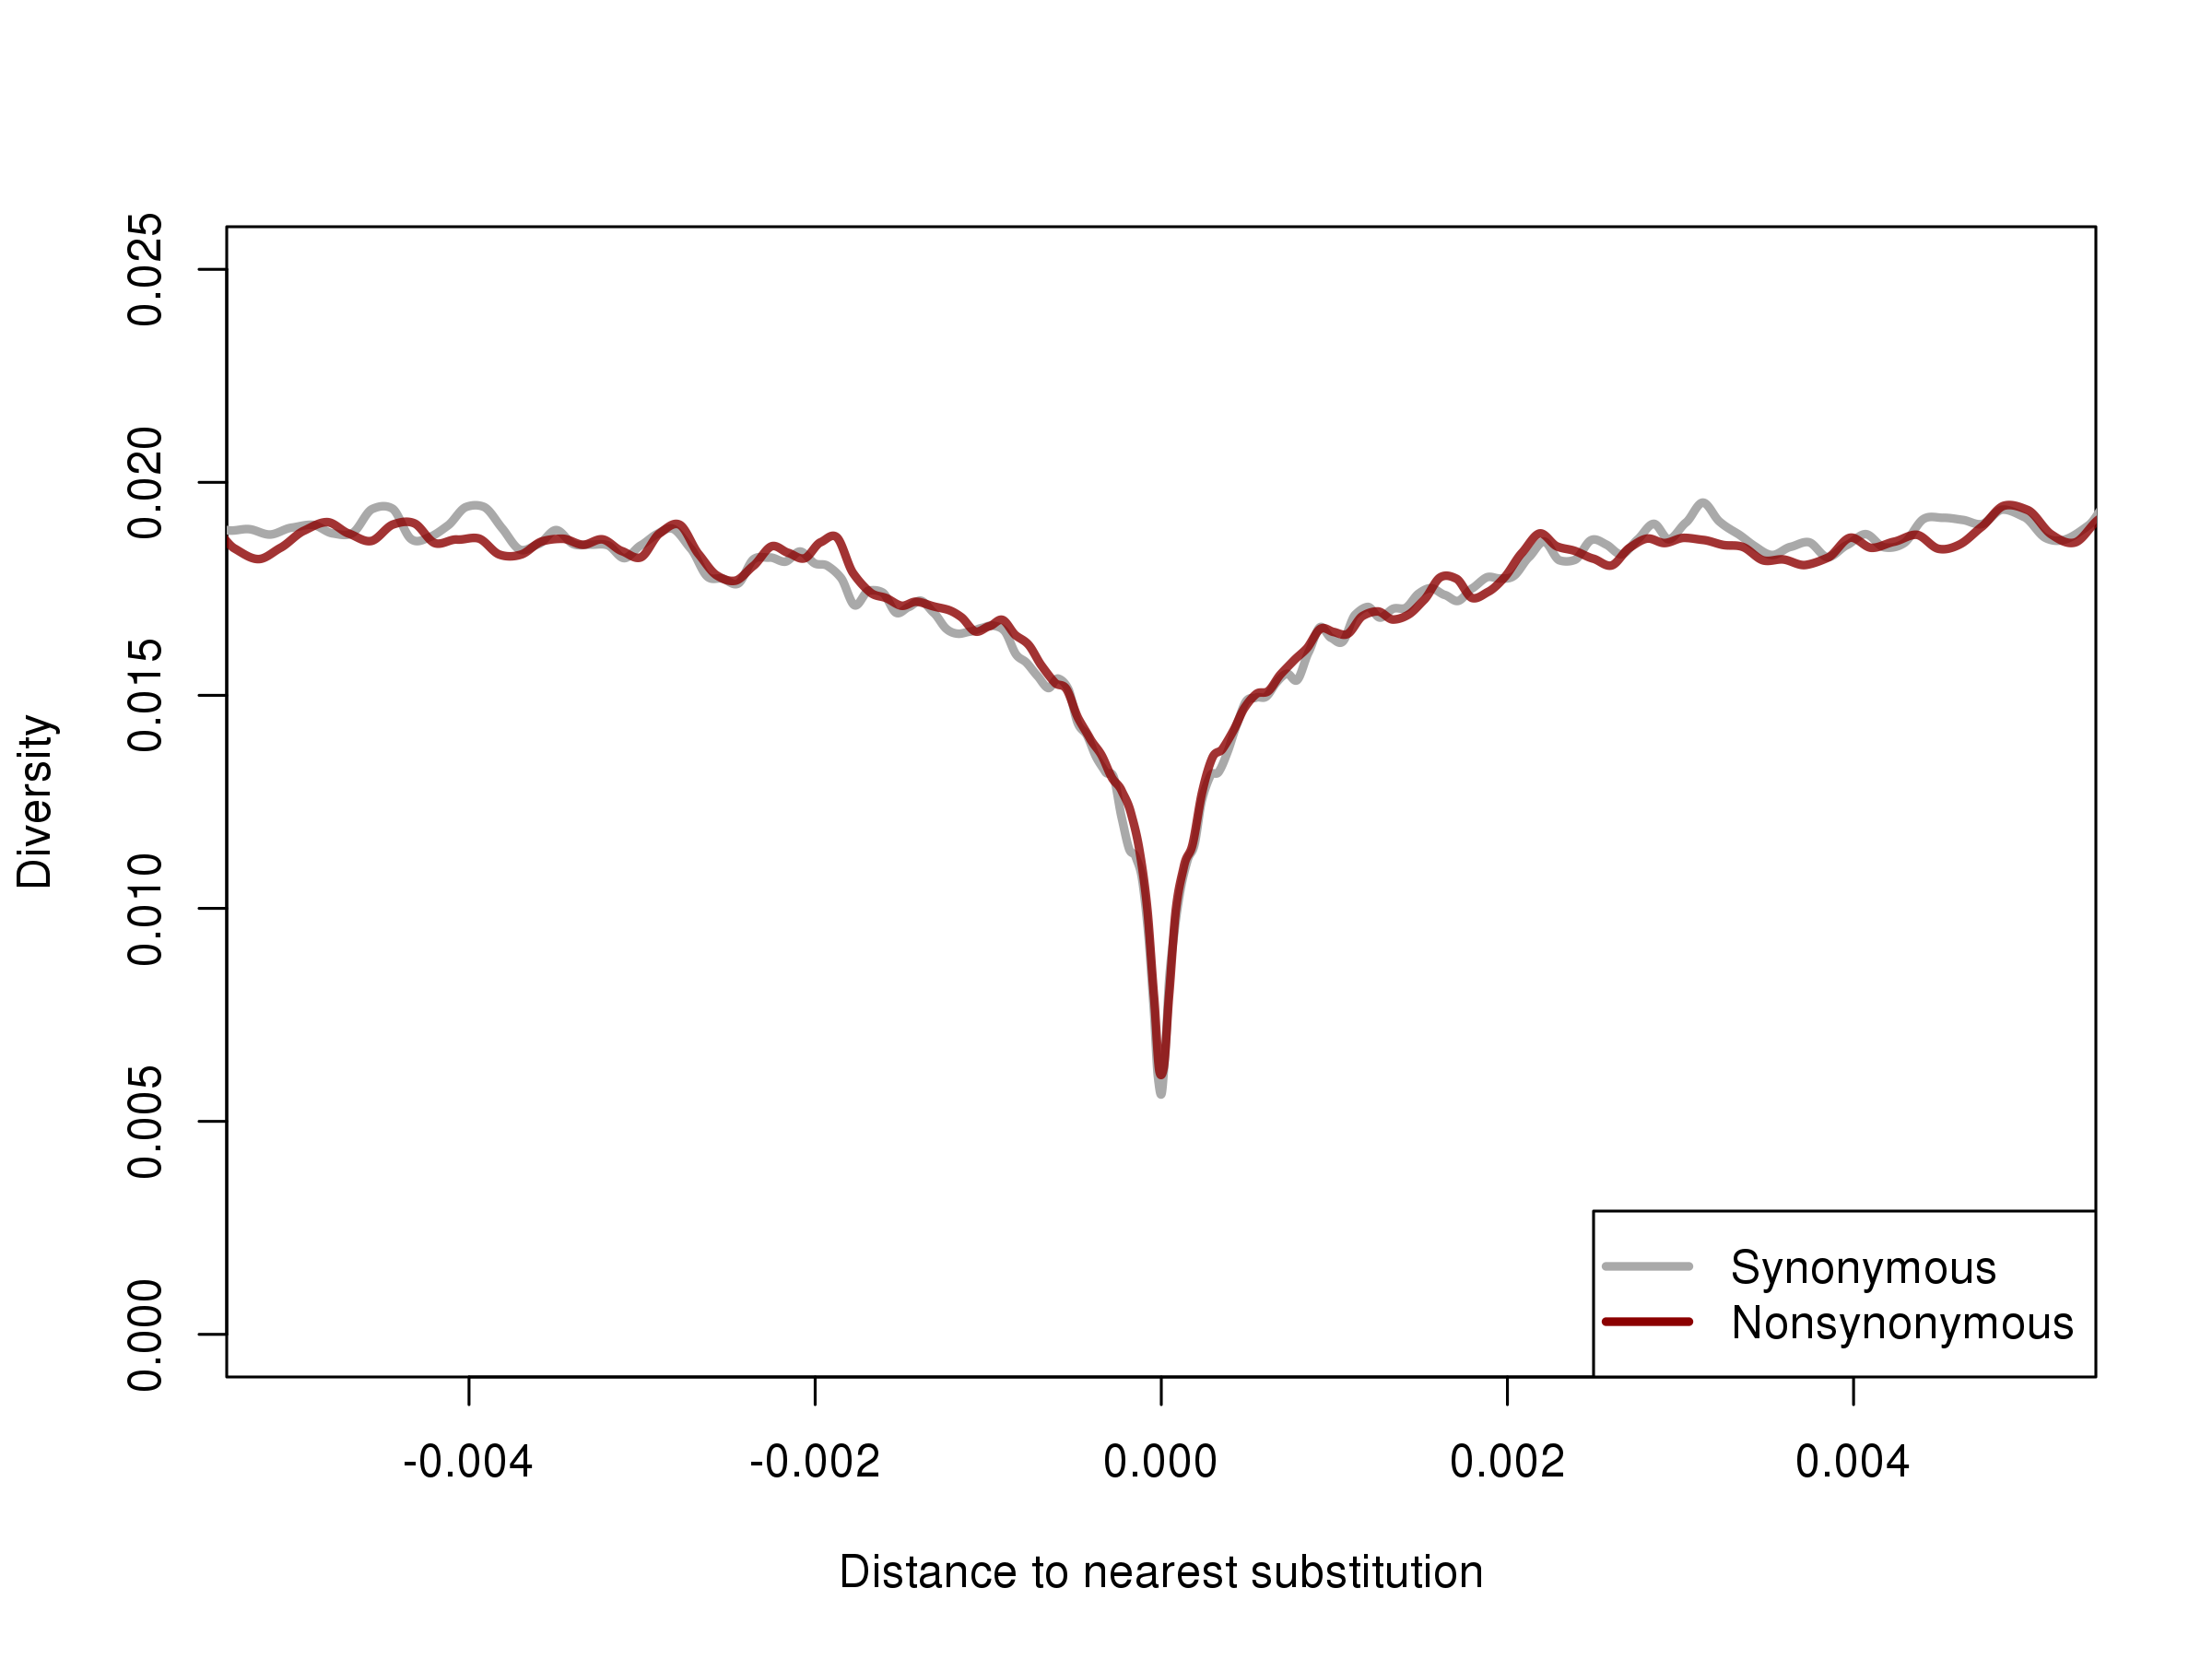
\includegraphics[width=\textwidth]{FigsAndFiles/plotDiversity_TvM_Singletons.png}
\caption{ Singleton diversity surrounding synonymous and nonsynonymous
  substitutions in maize. \label{sFig:singleton}}
\end{figure}
\clearpage


\begin{figure}
  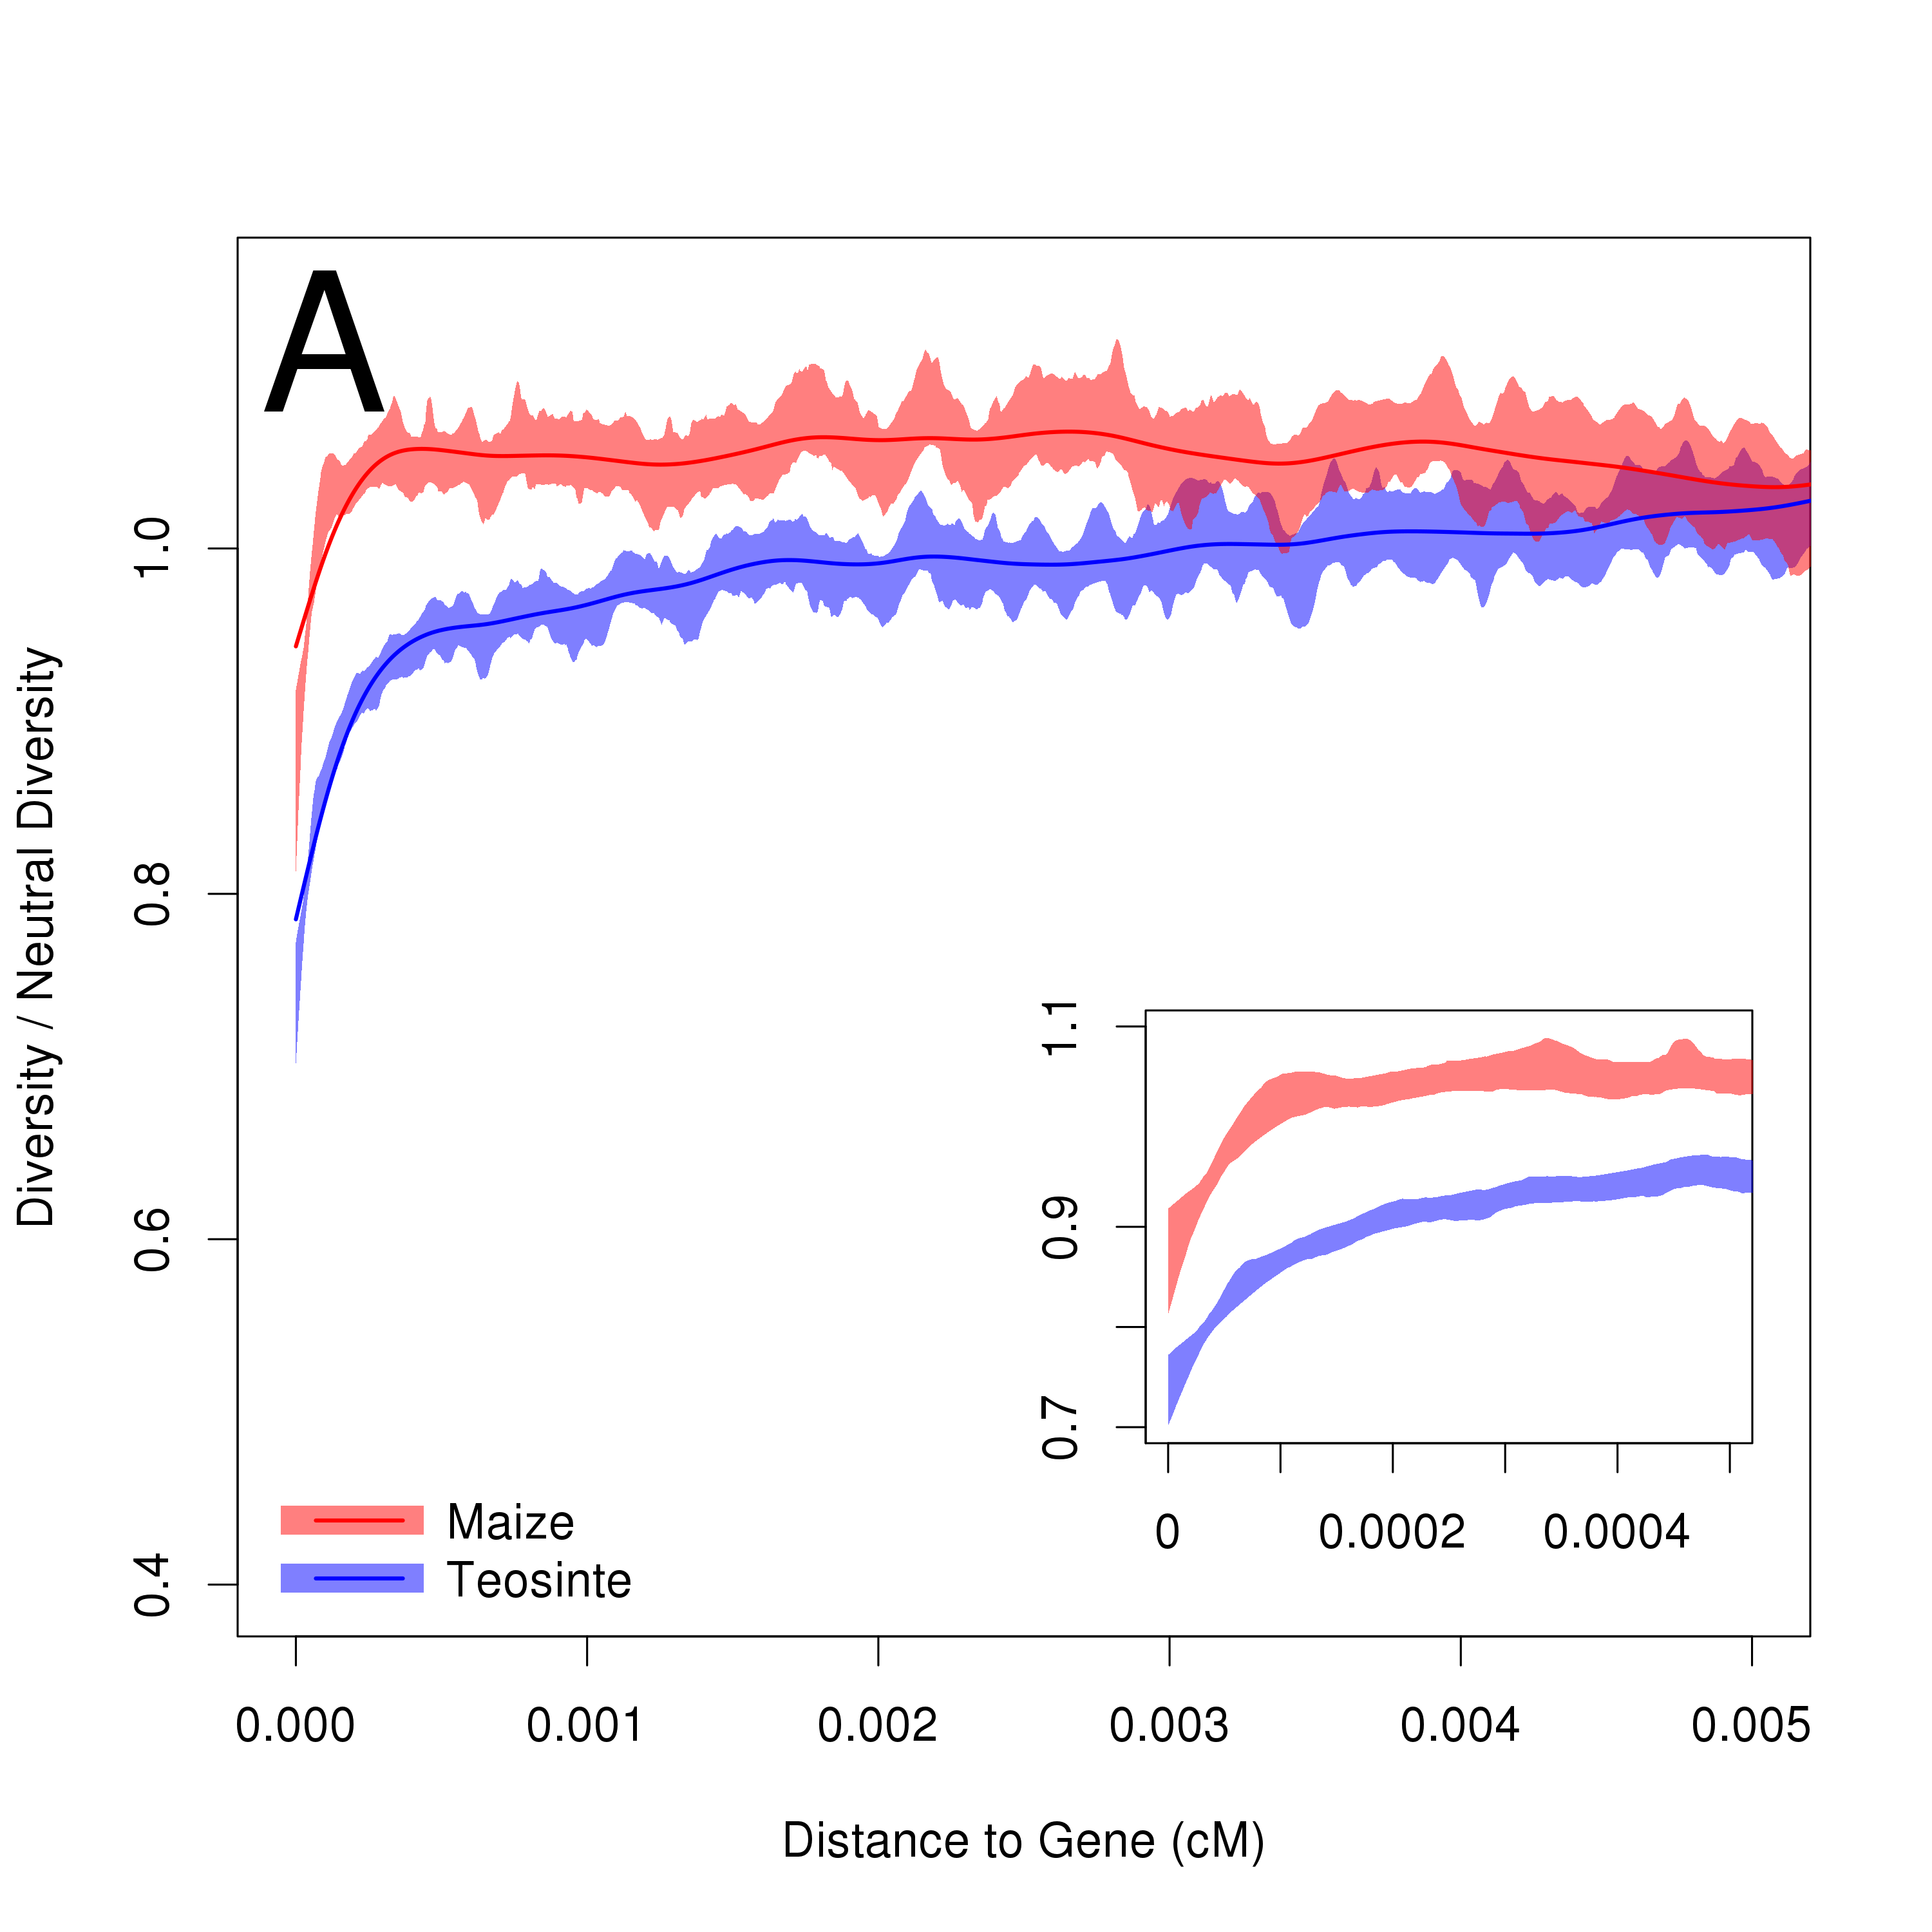
\includegraphics[width=.5\textwidth]{FigsAndFiles/distanceToGene_Unselected_manuscript.png}
    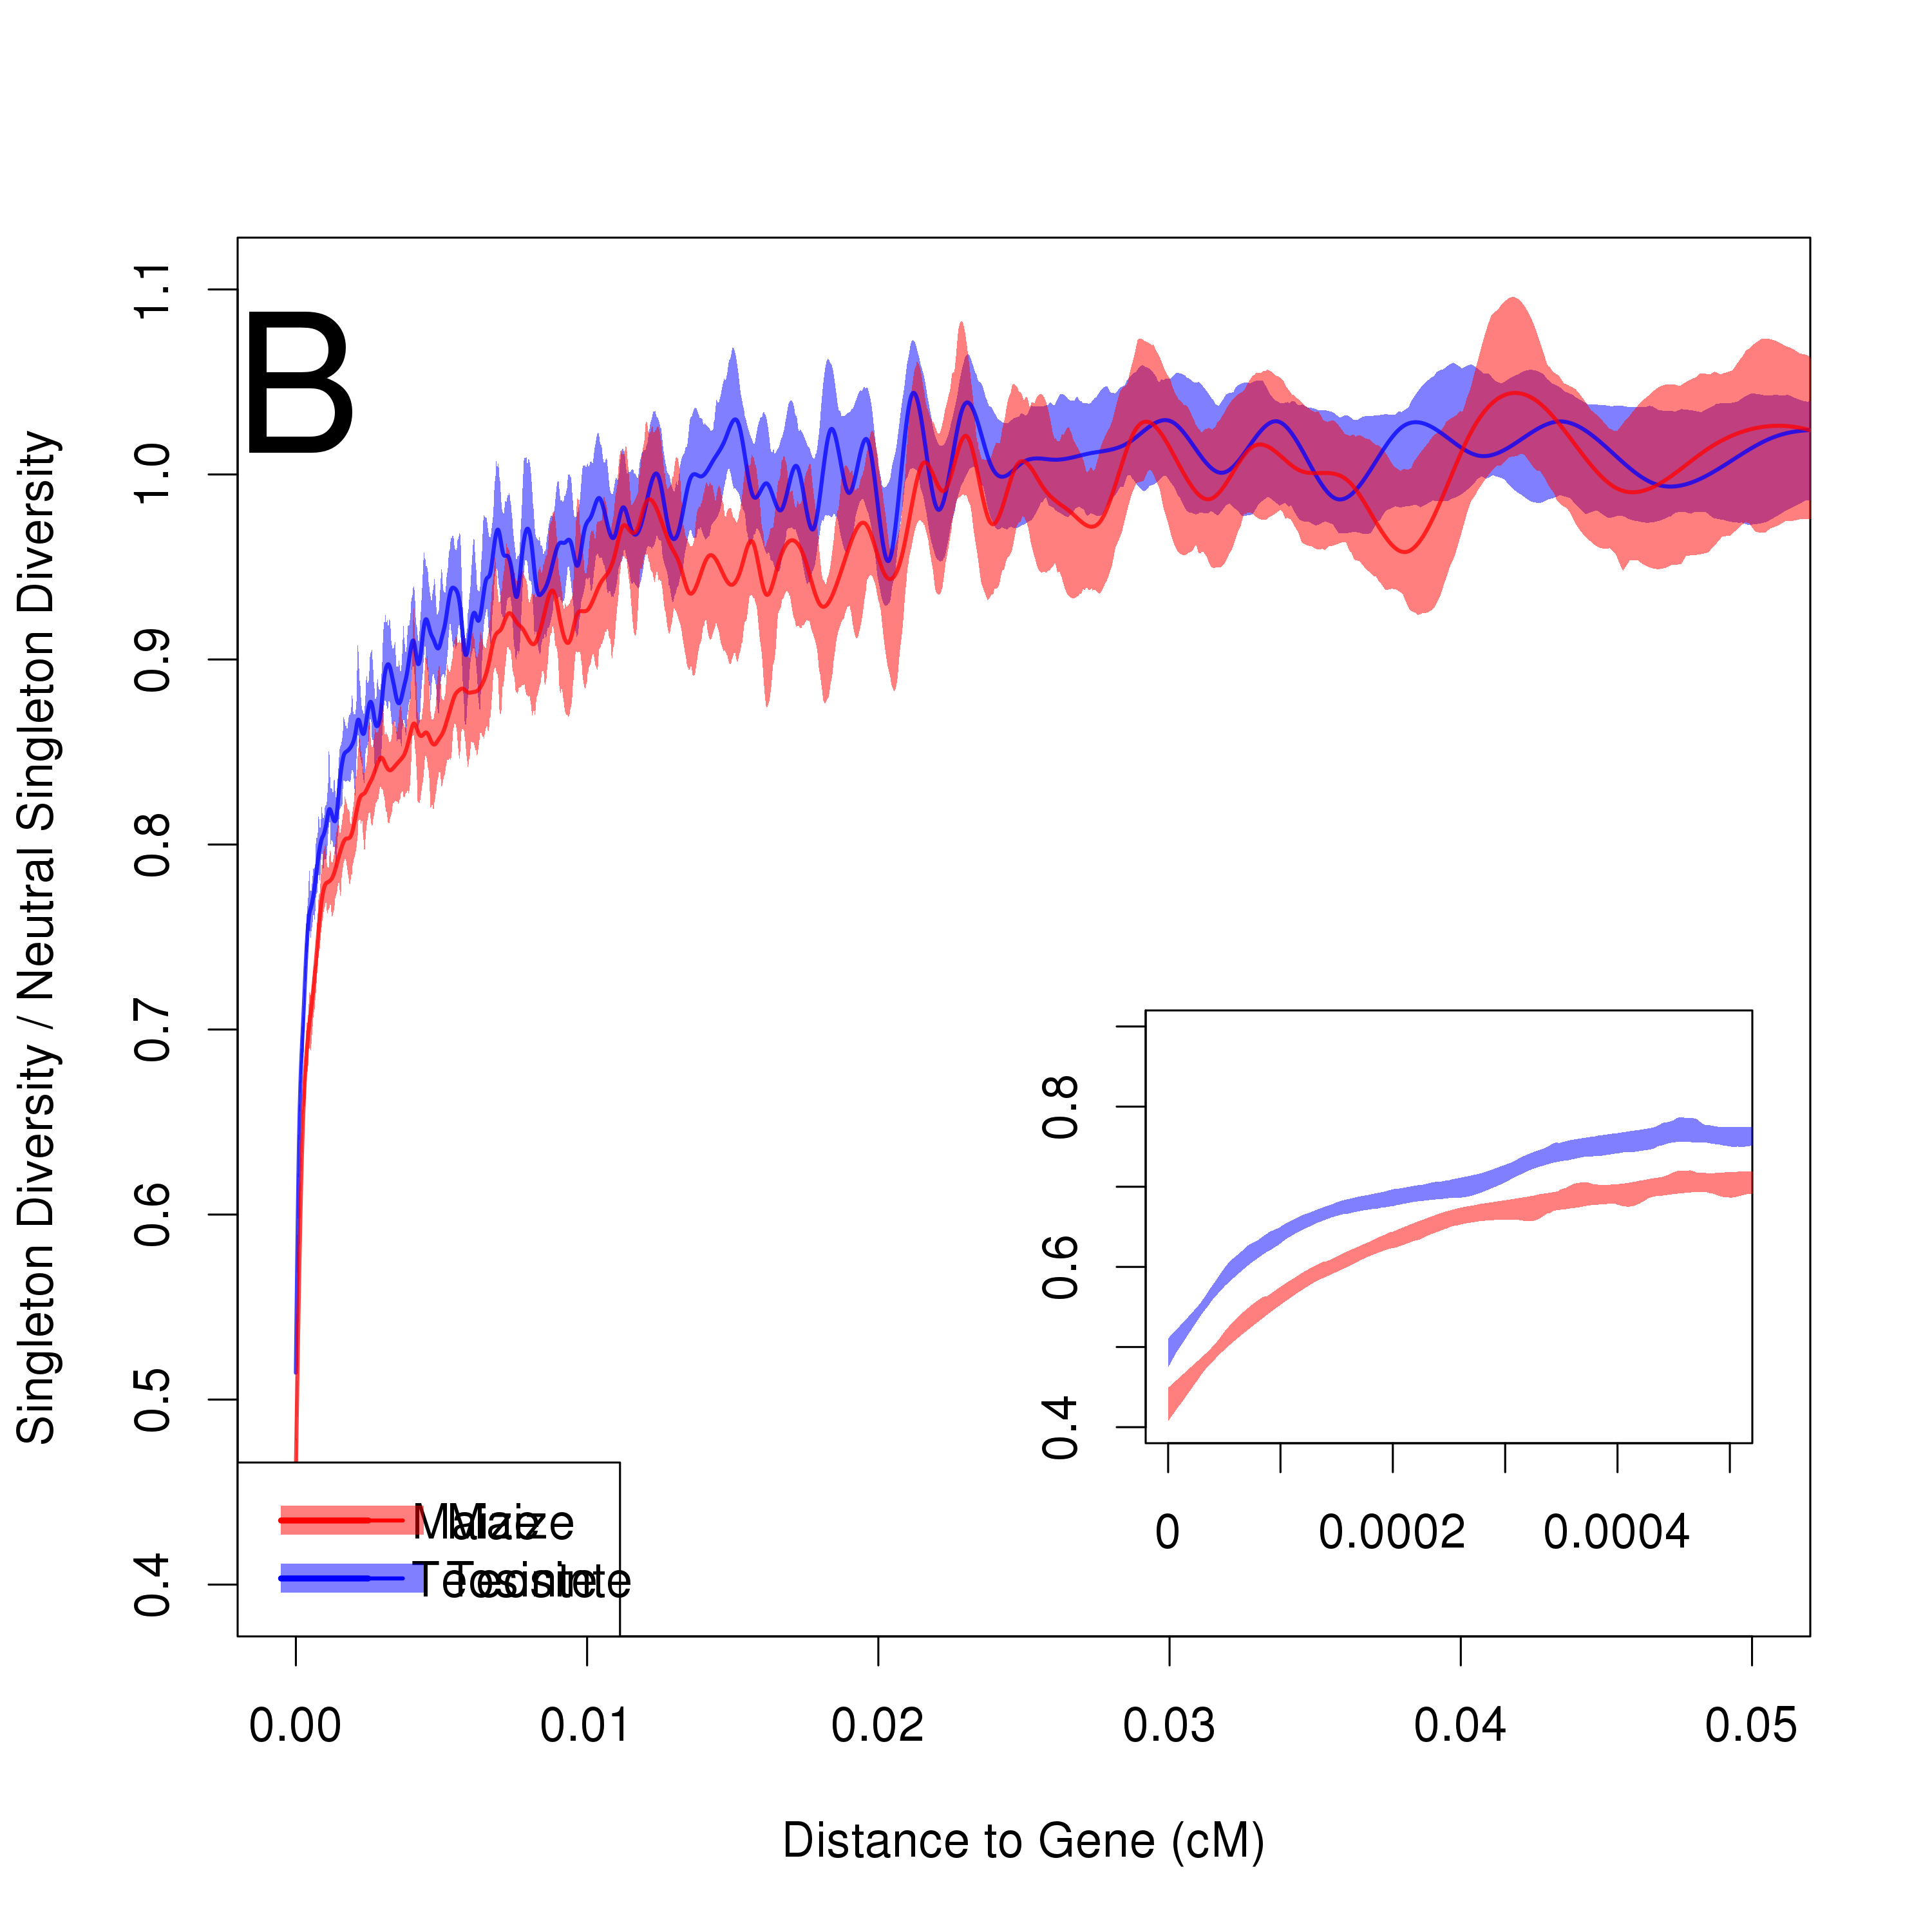
\includegraphics[width=.5\textwidth]{FigsAndFiles/distanceToGene_unselected_Singletons_manuscript.png}
\caption{ Relative level of diversity versus distance to the nearest gene, in maize and teosinte, based on only sites that do not show evidence of hard or soft sweeps according to H12. Two measures of diversity were investigated. {\bf A} displays pairwise diversity,
which is most influenced by intermediate frequency alleles and therefore depicts more ancient evolutionary patterns, and {\bf B} depicts singleton diversity, influenced by rare alleles and thus depicting evolutionary patterns in the recent past. Bootstrap-based 95\% confidence intervals are depicted via shading. Inset plots depict a smaller range on the x-axis. \label{sFig:H12}}
\end{figure}
\clearpage


\begin{figure}
  \begin{center}
  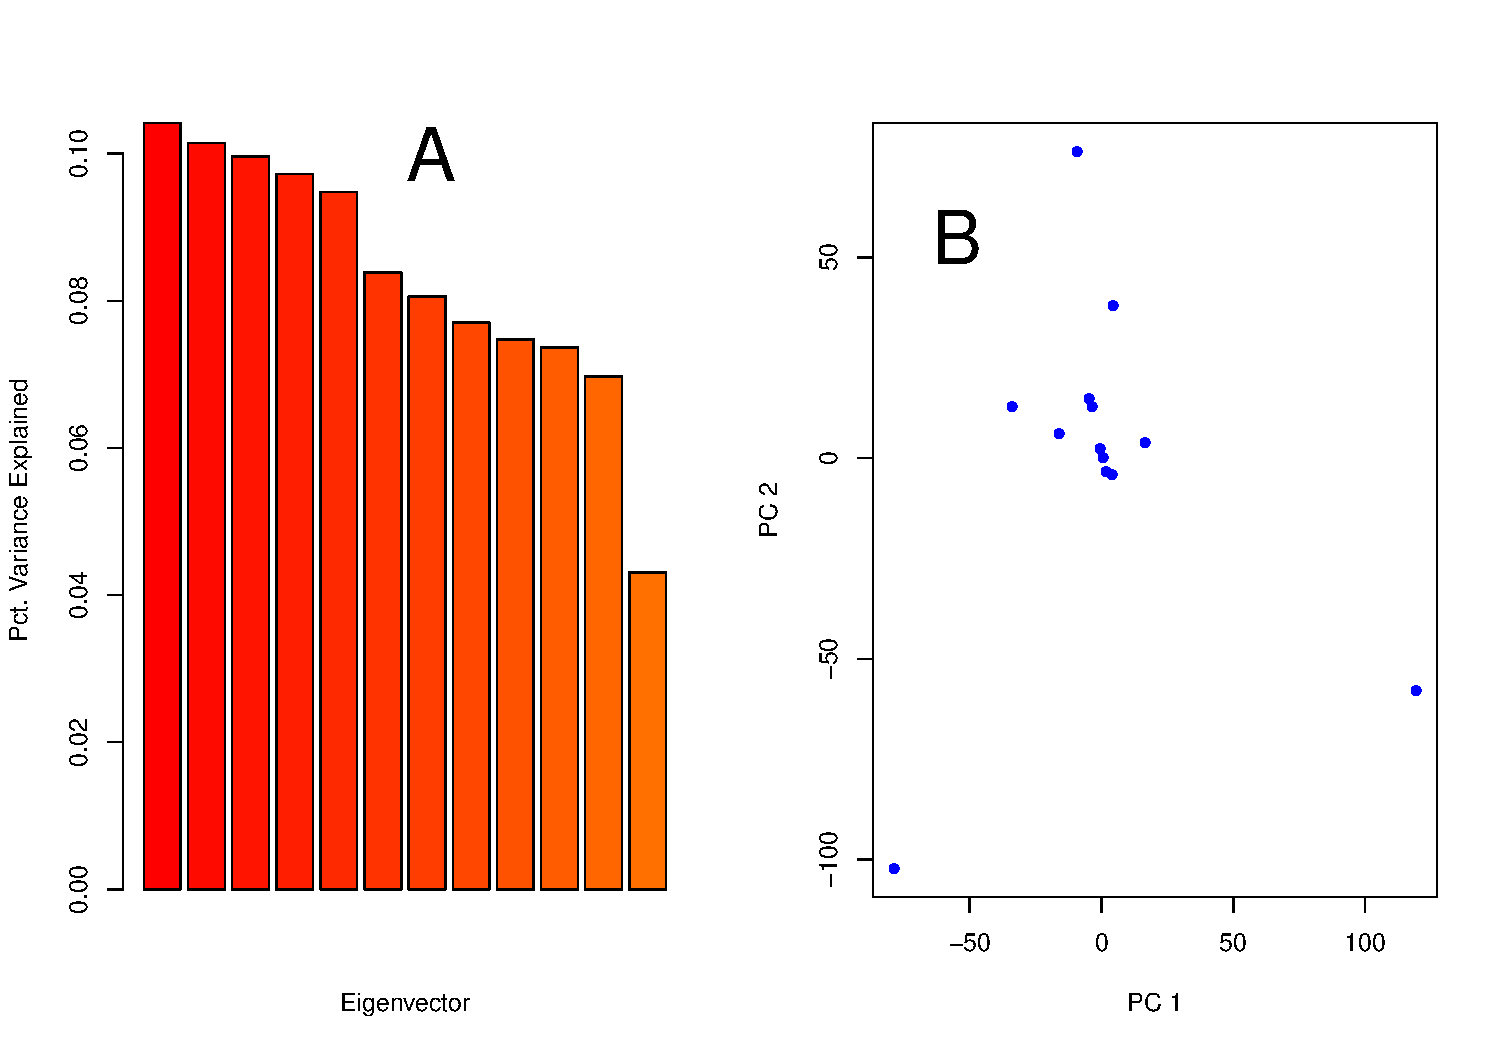
\includegraphics[width=.75\textwidth]{FigsAndFiles/tilPCA_july.pdf}\\
  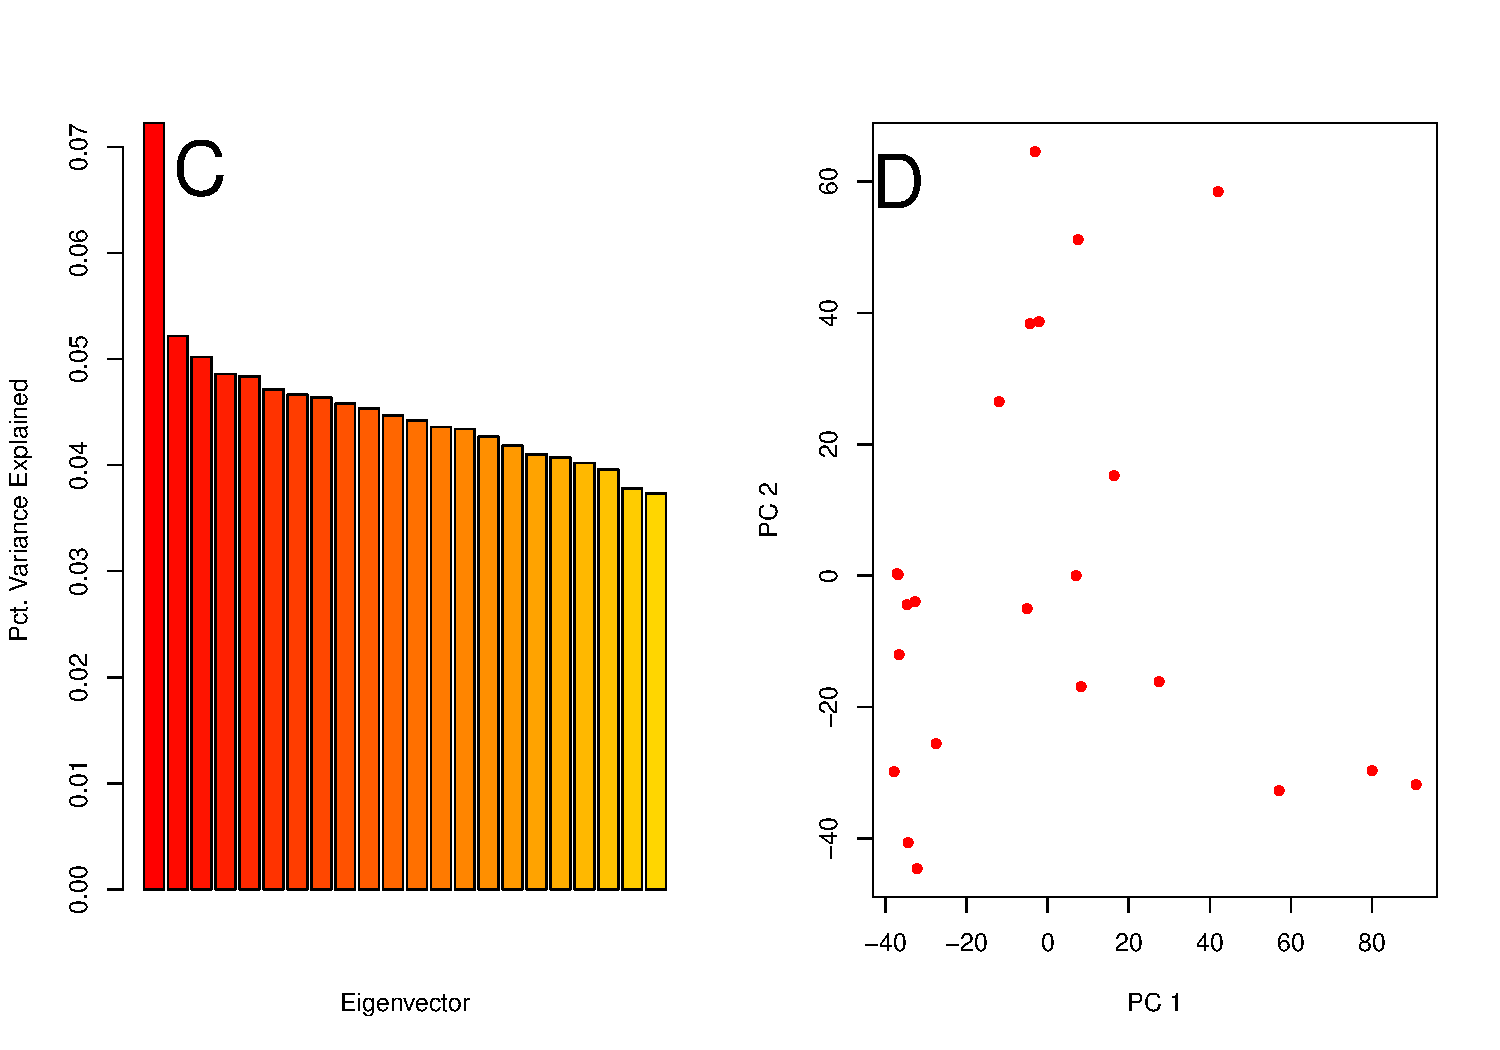
\includegraphics[width=.75\textwidth]{FigsAndFiles/bknPCA_july.pdf}\\
  \end{center}
  \caption{Principal component analysis of teosinte and maize individuals to ensure that no close relatives were inadvertantly included in our study. Plots are based on a random sample of 10,000 SNPs. {\bf A:} Percentage of total variance explained by each principal component for teosinte. {\bf B:} PC1 vs PC2 for all 13 teosinte individuals. {\bf C:} Percentage of total variance explained by each principal component for maize. {\bf D:} PC1 vs PC2 for all 23 maize individuals. \jri{need to fix letter label positions} \label{sFig:PCA}}
\end{figure}
\clearpage


\begin{figure}
%  \begin{center}
  \begin{tabular}{c|c}
    \bf Maize & \bf Teosinte \\ \hline \hline
    BKN009 &  TIL01 \\
    BKN010 & TIL02 \\
    BKN011 & TIL03 \\
    BKN014 & TIL04-TIP454 \\
    BKN015 & TIL07 \\
    BKN016 & TIL09 \\
    BKN017 & TIL10 \\
    BKN018 & TIL11 \\
    BKN019 & TIL12 \\
    BKN020 & TIL14-TIP498 \\
    BKN022 & TIL15 \\
    BKN023 & TIL16 \\
    BKN025 & TIL17 \\
    BKN026 & \\
    BKN027 & \\
    BKN029 & \\
    BKN030 & \\
    BKN031 & \\
    BKN032 & \\
    BKN033 & \\
    BKN034 & \\
    BKN035 & \\
    BKN040 & \\
  \end{tabular} 
%  \end{center}
  \caption{ A list of maize and teosinte individuals included in this study. Sequencing and details were previously described by \jri{cite chia and lemmon}   \label{sTab:list} }
\end{figure}
